 \documentclass[10pt,a4paper]{report}
\usepackage[utf8]{inputenc}
\usepackage{amsmath}
\usepackage{amsfonts}
\usepackage{amssymb}
\usepackage{amsthm}
\usepackage{hyperref}

\usepackage{multicol}
\usepackage{fancyhdr}
\usepackage[inline]{enumitem}
\usepackage{tikz}
\usepackage{tikz-cd}
\usetikzlibrary{calc}
\usetikzlibrary{shapes.geometric}
\usepackage[margin=0.5in]{geometry}
\usepackage{xcolor}

\usepackage{pgfplots}
\hypersetup{
    colorlinks=true,
    linkcolor=blue,
    filecolor=magenta,      
    urlcolor=cyan,
    pdftitle={Tensors},
    pdfpagemode=FullScreen,
    }

%\urlstyle{same}

\newcommand{\CLASSNAME}{Math 5050 -- Special Topics: Manifolds}
\newcommand{\STUDENTNAME}{Paul Carmody}
\newcommand{\ASSIGNMENT}{Assignment 5 }
\newcommand{\DUEDATE}{April 8, 2025}
\newcommand{\SEMESTER}{Spring 2025}
\newcommand{\SCHEDULE}{MW 12:30 - 1:45}
\newcommand{\ROOM}{Remote}

\newcommand{\MMN}{M_{m\times n}}
\newcommand{\FF}{\mathcal{F}}
\newcommand{\RANGE}{\text{range}}

\pagestyle{fancy}
\fancyhf{}
\chead{ \fancyplain{}{\CLASSNAME} }
%\chead{ \fancyplain{}{\STUDENTNAME} }
\rhead{\thepage}
\newcommand{\LET}{\text{Let }}
%\newcommand{\IF}{\text{if }}
\newcommand{\AND}{\text{ and }}
\newcommand{\OR}{\text{ or }}
\newcommand{\FORSOME}{\text{ for some }}
\newcommand{\FORALL}{\text{ for all }}
\newcommand{\WHERE}{\text{ where }}
\newcommand{\WTS}{\text{ WTS }}
\newcommand{\WLOG}{\text{ WLOG }}
\newcommand{\BS}{\backslash}
\newcommand{\DEFINE}[1]{\textbf{\emph{#1}}}
\newcommand{\IF}{$(\Rightarrow)$}
\newcommand{\ONLYIF}{$(\Leftarrow)$}
\newcommand{\ITH}{\textsuperscript{th} }
\newcommand{\FST}{\textsuperscript{st} }
\newcommand{\SND}{\textsuperscript{nd} }
\newcommand{\TRD}{\textsuperscript{rd} }
\newcommand{\INV}{\textsuperscript{-1} }


%%%%%%%
% derivatives
%%%%%%%

\newcommand{\PART}[2]{\frac{\partial #1}{\partial #2}}
\newcommand{\SPART}[2]{\frac{\partial^2 #1}{\partial #2^2}}
\newcommand{\DERIV}[2]{\frac{d #1}{d #2}}
\newcommand{\LAPLACIAN}[1]{\frac{\partial^2 #1}{\partial x^2} + \frac{\partial^2 #1}{\partial y^2}}

%%%%%%%
% sum, product, union, intersections
%%%%%%%

\newcommand{\SUM}[2]{\underset{#1}{\overset{#2}{\sum}}}
\newcommand{\PROD}[2]{\underset{#1}{\overset{#2}{\prod}}}
\newcommand{\UNION}[2]{\underset{#1}{\overset{#2}{\bigcup}}}
\newcommand{\INTERSECT}[2]{\underset{#1}{\overset{#2}{\bigcap}}}
\newcommand{\FSUM}{\SUM{n=-\infty}{\infty}}
       

%%%%%%%
% supremum and infimum
%%%%%%%

\newcommand{\SUP}[1]{\underset{#1}\sup \,}
\newcommand{\INF}[1]{\underset{#1}\inf \,}
\newcommand{\MAX}[1]{\underset{#1}\max \,}
\newcommand{\MIN}[1]{\underset{#1}\min \,}

%%%%%%%
% infinite sums, limits
%%%%%%%

\newcommand{\SUMK}{\SUM{k=1}{\infty}}
\newcommand{\SUMN}{\SUM{n=1}{\infty}}
\newcommand{\SUMKZ}{\SUM{k=0}{\infty}}
\newcommand{\LIM}[1]{\underset{#1}\lim\,}
\newcommand{\IWOB}[1]{\LIM{#1 \to \infty}}
\newcommand{\LIMK}{\IWOB{k}}
\newcommand{\LIMN}{\IWOB{n}}
\newcommand{\LIMX}{\IWOB{x}}
\newcommand{\NIWOB}{\LIM{n \to \infty}}
\newcommand{\LIMSUPK}{\underset{k\to\infty}\limsup \,}
\newcommand{\LIMSUPN}{\underset{n\to\infty}\limsup \,}
\newcommand{\LIMINFK}{\underset{k\to\infty}\liminf \,}
\newcommand{\LIMINFN}{\underset{n\to\infty}\liminf \,}
\newcommand{\ROOTRULE}[1]{\LIMSUPK \BARS{#1}^{1/k}}

\newcommand{\CUPK}{\bigcup_{k=1}^{\infty}}
\newcommand{\CAPK}{\bigcap_{k=1}^{\infty}}
\newcommand{\CUPN}{\bigcup_{n=1}^{\infty}}
\newcommand{\CAPN}{\bigcap_{n=1}^{\infty}}

%%%%%%%
% number systems (real, rational, etc.)
%%%%%%%

\newcommand{\REALS}{\mathbb{R}}
\newcommand{\RATIONALS}{\mathbb{Q}}
\newcommand{\IRRATIONALS}{\REALS \backslash \RATIONALS}
\newcommand{\INTEGERS}{\mathbb{Z}}
\newcommand{\NUMBERS}{\mathbb{N}}
\newcommand{\COMPLEX}{\mathbb{C}}
\newcommand{\DISC}{\mathbb{D}}
\newcommand{\HPLANE}{\mathbb{H}}

\newcommand{\R}{\mathbb{R}}
\newcommand{\Q}{\mathbb{Q}}
\newcommand{\Z}{\mathbb{Z}}
\newcommand{\N}{\mathbb{N}}
\newcommand{\C}{\mathbb{C}}
\newcommand{\T}{\mathbb{T}}
\newcommand{\COUNTABLE}{\aleph_0}
\newcommand{\UNCOUNTABLE}{\aleph_1}


%%%%%%%
% Arithmetic/Algebraic operators
%%%%%%%


\DeclareMathOperator{\MOD}{mod}
%\newcommand{\MOD}[1]{\mod #1}
\newcommand{\BAR}[1]{\overline{#1}}
\newcommand{\LCM}{\text{ lcm}}
\newcommand{\ZMOD}[1]{\Z/#1\Z}
\DeclareMathOperator{\VAR}{Var}
%%%%%%%
% complex operators
%%%%%%%

\DeclareMathOperator{\RR}{Re}
%\newcommand{\RE}{\text{Re}}
\DeclareMathOperator{\IM}{Im}
%\newcommand{\IM}{\text{Im}}
\newcommand{\CONJ}[1]{\overline{#1}}
\DeclareMathOperator{\LOG}{Log}
%\newcommand{\LOG}{\text{ Log }}
\newcommand{\RES}[2]{\underset{#1}{\text{res}} #2}

%%%%%%%
% Group operators
%%%%%%%

\newcommand{\AUT}{\text{Aut}\,}
\newcommand{\KER}{\text{ker}\,}
\newcommand{\END}{\text{End}}
\newcommand{\HOM}{\text{Hom}}
\newcommand{\CYCLE}[1]{(\begin{array}{cccccccccc}
		#1
	\end{array})}
\newcommand{\SUBGROUP}{\underset{\text{group}}\subseteq}	
%\newcommand{\SUBGROUP}{\subseteq_g}
\newcommand{\SUBRING}{\underset{\text{ring}}\subseteq}
\newcommand{\SUBMOD}{\underset{\text{mod}}\subseteq}
\newcommand{\SUBFIELD}{\underset{\text{field}}\subseteq}
\newcommand{\ISO}{\underset{\text{iso}}\longrightarrow}
\newcommand{\HOMO}{\underset{\text{homo}}\longrightarrow}

%%%%%%%
% grouping (parenthesis, absolute value, square, multi-level brackets).
%%%%%%%

\newcommand{\PAREN}[1]{\left (\, #1 \,\right )}
\newcommand{\BRACKET}[1]{\left \{\, #1 \,\right \}}
\newcommand{\SQBRACKET}[1]{\left [\, #1 \,\right ]}
\newcommand{\ABRACKET}[1]{\left \langle\, #1 \,\right \rangle}
\newcommand{\BARS}[1]{\left |\, #1 \,\right |}
\newcommand{\DBARS}[1]{\left \| \, #1 \,\right \|}
\newcommand{\LBRACKET}[1]{\left \{ #1 \right .} 
\newcommand{\RBRACKET}[1]{\left . #1 \right \]}
\newcommand{\RBAR}[1]{\left . #1 \, \right |}
\newcommand{\LBAR}[1]{\left | \, #1 \right .}
\newcommand{\BLBRACKET}[2]{\BRACKET{\RBAR{#1}#2}}
\newcommand{\GEN}[1]{\ABRACKET{#1}}
\newcommand{\BINDEF}[2]{\LBRACKET{\begin{array}{ll}
     #1\\
     #2
\end{array}}}

%%%%%%%
% Fourier Analysis
%%%%%%%

\newcommand{\ONEOTWOPI}{\frac{1}{2\pi}}
\newcommand{\FHAT}{\hat{f}(n)}
\newcommand{\FINT}{\int_{-\pi}^\pi}
\newcommand{\FINTWO}{\int_{0}^{2\pi}}
\newcommand{\FSUMN}[1]{\SUM{n=-#1}{#1}}
%\newcommand{\FSUM}{\SUMN{\infty}}
\newcommand{\EIN}[1]{e^{in#1}}
\newcommand{\NEIN}[1]{e^{-in#1}}
\newcommand{\INTALL}{\int_{-\infty}^{\infty}}
\newcommand{\FTINT}[1]{\INTALL #1 e^{2\pi inx\xi} dx}
\newcommand{\GAUSS}{e^{-\pi x^2}}

%%%%%%%
% formatting 
%%%%%%%

\newcommand{\LEFTBOLD}[1]{\noindent\textbf{#1}}
\newcommand{\SEQ}[1]{\{#1\,\}}
\newcommand{\WIP}{\footnote{work in progress}}
\newcommand{\QED}{\hfill\square}
\newcommand{\ts}{\textsuperscript}
\newcommand{\HLINE}{\noindent\rule{7in}{1pt}\\}

%%%%%%%
% Mathematical note taking (definitions, theorems, etc.)
%%%%%%%

\newcommand{\REM}{\noindent\textbf{\\Remark: }}
\newcommand{\DEF}{\noindent\textbf{\\Definition: }}
\newcommand{\THE}{\noindent\textbf{\\Theorem: }}
\newcommand{\COR}{\noindent\textbf{\\Corollary: }}
\newcommand{\LEM}{\noindent\textbf{\\Lemma: }}
\newcommand{\PROP}{\noindent\textbf{\\Proposition: }}
\newcommand{\PROOF}{\noindent\textbf{\\Proof: }}
\newcommand{\EXP}{\noindent\textbf{\\Example: }}
\newcommand{\TRICKS}{\noindent\textbf{\\Tricks: }}


%%%%%%%
% text highlighting
%%%%%%%

\newcommand{\B}[1]{\textbf{#1}}
\newcommand{\CAL}[1]{\mathcal{#1}}
\newcommand{\UL}[1]{\underline{#1}}

%%%%%%
% Linear Algebra
%%%%%%

\newcommand{\COLVECTOR}[1]{\PAREN{\begin{array}{c}
#1
\end{array} }}
\newcommand{\TWOXTWO}[4]{\PAREN{ \begin{array}{c c} #1&#2 \\ #3 & #4 \end{array} }}
\newcommand{\THREEXTHREE}[9]{\PAREN{ \begin{array}{c c c} #1&#2&#3 \\ #4 & #5 & #6 \\ #7 & #8 & #9 \end{array} }}
\newcommand{\NXN}{\PAREN{ \begin{array}{c c c c} 
			a_{11} & a_{12} & \cdots & a_{1n} \\
			a_{21} & a_{22} & \cdots & a_{2n} \\
			\vdots & \vdots & \ddots & a_{1n} \\
			a_{n1} & a_{n2} & \cdots & a_{nn} \\
		\end{array} }}
\newcommand{\SLR}{SL_2(\R)}
\newcommand{\GLR}{GL_2(\R)}
\DeclareMathOperator{\TR}{tr}
\DeclareMathOperator{\BIL}{Bil}
\DeclareMathOperator{\SPAN}{span}

%%%%%%%
%  White space
%%%%%%%

\newcommand{\BOXIT}[1]{\noindent\fbox{\parbox{\textwidth}{#1}}}


\newtheorem{theorem}{Theorem}[section]
\newtheorem{corollary}{Corollary}[theorem]
\newtheorem{lemma}[theorem]{Lemma}

\theoremstyle{definition}
\newtheorem{definition}[theorem]{Definition}
\newtheorem{prop}[theorem]{Proposition}

\theoremstyle{remark}
\newtheorem{remark}[theorem]{Remark}
\newtheorem{example}[theorem]{Example}
%\newtheorem*{proof}[theorem]{Proof}



\newcommand{\RED}[1]{\textcolor{red}{#1}}
\newcommand{\BLUE}[1]{\textcolor{blue}{#1}}

\begin{document}

\begin{center}
	\Large{\CLASSNAME -- \SEMESTER} \\
	\large{ w/Professor Berchenko-Kogan}
\end{center}
\begin{center}
	\STUDENTNAME \\
	\ASSIGNMENT -- \DUEDATE\\
\end{center} 

\noindent Section 5 problems 3 and 5 \\

\noindent\textbf{5.3 Charts on a Sphere.}

Let $S^2$ be the unit sphere 
\begin{align*}
	x^2+y^2+z^2=1
\end{align*}in $\R^3$.  	In $S^2$ the six charts corresponding to the siz hemspheres -- the front, rear, right, let, upper and lower hemisphere (Figure 5.11):
\begin{align*}
	U_1 &= \{(x,y,z) \in S^2\,|\, x > 0\}, \; \phi_1(x,y,z) = (y,z) \\
	U_2 &= \{(x,y,z) \in S^2\,|\, x < 0\}, \; \phi_2(x,y,z) = (y,z) \\
	U_3 &= \{(x,y,z) \in S^2\,|\, y > 0\}, \; \phi_3(x,y,z) = (x,z) \\
	U_4 &= \{(x,y,z) \in S^2\,|\, y < 0\}, \; \phi_4(x,y,z) = (x,z) \\
	U_5 &= \{(x,y,z) \in S^2\,|\, z > 0\}, \; \phi_5(x,y,z) = (x,y) \\
	U_6 &= \{(x,y,z) \in S^2\,|\, z < 0\}, \; \phi_6(x,y,z) = (x,y) 
\end{align*}Describe the domain of $\phi_4(U_{14})$ of $\phi_1\circ \phi_4^{-1}$ and show that $\phi_1\circ\phi_4^{-1}$ is $ C^\infty$ on $\phi_4(U_{14})$.  Do the same for $\phi_6\circ \phi_1^{-1}$.

\BLUE{
\begin{align*}
	U_{14} &= U_1 \cap U_4 \\
	&= \{(x,y,z) \in S^2\,|\, x > 0\} \cap \{(x,y,z) \in S^2\,|\, y < 0\} \\
	&= \{(x,y,z) \in S^2\,|\, x > 0 \AND y<0\}
\end{align*}This is the half hemisphere typically thought of as to the right and above and below the the plane of the equator.
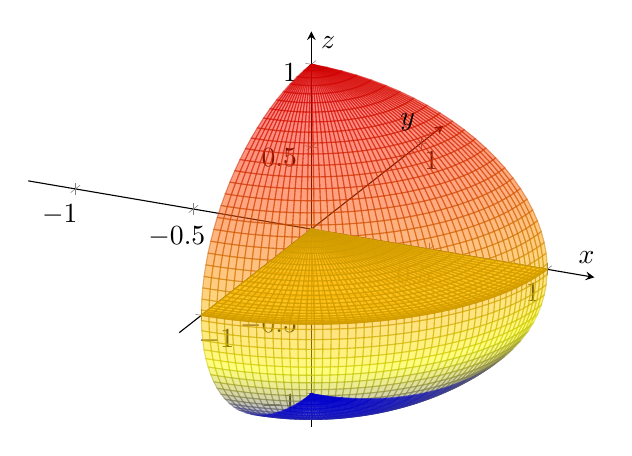
\begin{tikzpicture}
  \begin{axis}[width=\textwidth,
      samples=50,domain=90:180,y domain=90:270,
      xmin=-1.2,xmax=1.2,ymin=-1.2,ymax=1.2,zmin=-1.2,zmax=1.2,
      xlabel={$x$},ylabel={$y$},zlabel={$z$},
    axis lines=center]
    \addplot3[surf,opacity=0.5]
    ({cos(x)*cos(y)}, {sin(x)*cos(y)}, {sin(y)});
%    ({cos(x)*cos(y)}, {sin(x)*cos(y)}, {sin(y)});
	\addplot3[surf, opacity=0.5]
    ({cos(x)*cos(y)}, {sin(x)*cos(y)}, 0);
  \end{axis}
\end{tikzpicture}\\
Show that $\phi_1 \circ \phi_4^{-1}$ is $C^\infty$.  We start by given any $(x,y)$ we can can see that $\phi_4^{-1} \mapsto (x,y,z) \subset \R^3$ and $\phi_1 \circ \phi_4^{-1}(x,y) \in (y,z)$ for any arbitrary third coordinate $z$.  The first coordinate maps open sets in $y$ to theirself and the second coordinate is open as it maps to all of $z$.  Thus, $\phi_1 \circ \phi_4^{-1}$ is $C^\infty$.\\
\\
Show the same for $\phi_6 \circ \phi_1^{-1}$.  First we describe $U_{61}$.
\begin{align*}
	U_{61} &= U_6 \cap U_1 \\
	&= \{(x,y,z) \in S^2\,|\, z < 0\} \cap \{(x,y,z) \in S^2\,|\, x > 0\} \\
	&= \{(x,y,z) \in S^2\,|\, x > 0 \AND z<0\}
\end{align*}This is the half hemisphere typically thought of as below the plane passing through the equator and to the right.  (Note that this picture shows some parts of the surface as $x<0$ which is an error.)\\
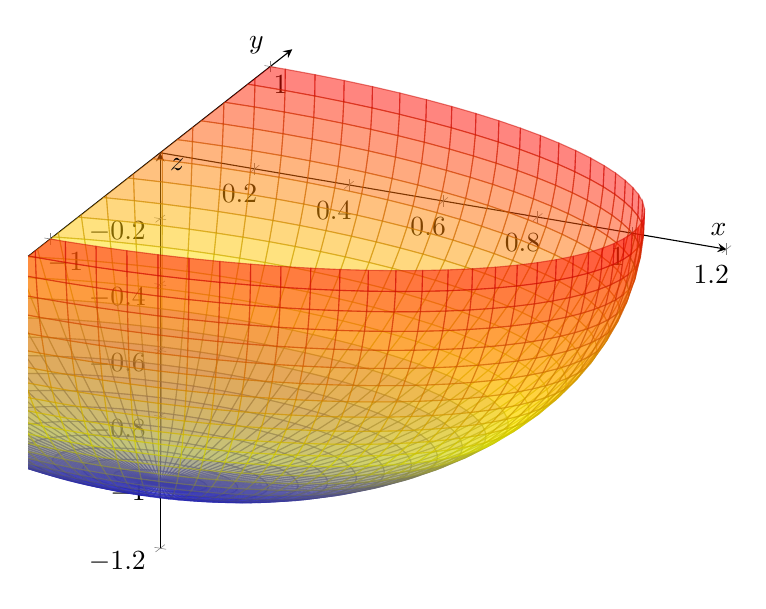
\begin{tikzpicture}
  \begin{axis}[width=\textwidth,
      samples=50,domain=0:180,y domain=180:360,
      xmin=0,xmax=1.2,ymin=-1.2,ymax=1.2,zmin=-1.2,zmax=0,
      xlabel={$x$},ylabel={$y$},zlabel={$z$},
    axis lines=center]
%	\addplot3[surf, opacity=0.5]
%    (0, {sin(x)*cos(y)}, {sin(y)});
    \addplot3[surf,opacity=0.5]
    ({cos(x)*cos(y)}, {sin(x)*cos(y)}, {sin(y)});
  \end{axis}
\end{tikzpicture}\\
Show that $\phi_6 \circ \phi_1^{-1}$ is $C^\infty$.  We start by given any $(y,z)$ we can can see that $\phi_1^{-1} \mapsto (x,y,z) \subset \R^3$ and $\phi_6 \circ \phi_1^{-1}(y,z) \in (y,z)$.  Thus any open set in $y$ or $z$ will be mapped to opened to themselves through $\phi_6 \circ \phi_1^{-1}$.  Both coordinates map open sets to semi-circles on planes parallel to the $y-z$ plane and $x>0$.  Thus, $\phi_6 \circ \phi_1^{-1}$ is $C^\infty$.
}

\newpage
\noindent\textbf{5.5 An Atlas for a Product Manifold.}

\textbf{Propostion 5.18 (an Atlas for a Product Manifold).}  If $\{(U_\alpha, \phi_\alpha)\}$ and $\{(V_i,\psi_i)\}$ are $C^\infty$ atlases for the manifold $M$ and $N$ with dimension $m$ and $n$, respectively, then the collection 
\begin{align*}
	\Phi=\BRACKET{\PAREN{U_\alpha\times V_i,\;\  \phi_\alpha\times \psi_i\,:\,U_\alpha\times V_i \to \R^m\times \R^n }}
\end{align*}of charts is a $C^\infty$ atlas $M\times N$.  Therefore, $M\times N$ is a $C^\infty$ smooth manifold of dimension $m+n$.\\

% Need to show:
% 	1) $M$ is Hausdorff and Second Countable
%   2) $M$ has a $C^\infty$ atlas.

\BLUE{\noindent Need to show, for some $\alpha, i$
\begin{enumerate}
	\item $x \in M \times N \implies x \in U_\alpha \times V_i$.
	\begin{align*}
		x \in M \times N &\implies \exists u \in M, v \in N \to x = (u,v) \\
		\AND \exists\, \alpha, i &\to u \in U_\alpha, v \in V_i \\
		\therefore x &= (u,v) \in U_\alpha \times V_i \in \Phi
	\end{align*}
	\item $x \in  U_\alpha \times V_i \implies x \in M \times N$. 
	\begin{align*}
		x \in  U_\alpha \times V_i &\implies \exists\, u\in U_\alpha, v \in V_i \to x = (u,v)\\
		u \in U_\alpha &\implies u \in M \AND v \in V_i \implies v \in N\\
		\therefore (u,v) \in M\times N &\implies x \in M \times N
	\end{align*}
	\item Furthmore, any two functions of the form $\phi_\alpha \times \psi_i$ are compatible.
	\begin{align*}
	\LET (x,y) &\in U_\alpha \times V_i \AND (u,v) \in U_\beta \times V_j  \\
	\text{define } \Theta_1 &: \phi_\alpha\times \psi_i(x,y)\to \R^m\times \R^n  \AND \Theta_2 : \phi_\beta\times \psi_j(u,v)\to \R^m\times \R^n  
\end{align*}for some $\alpha, \beta$ and $i, j$.  Since, $\phi_\alpha$ is compatible with $\phi_\beta$ and $\psi_i$ is compatible with $\psi_j$ so is $\Theta_1$ compatible with $\Theta_2$.  Since $\phi_\alpha, \phi_\beta, \psi_i, \psi_j \in C^\infty$ so is $\Theta_1, \Theta_2 \in C^\infty$.  Further, for any $x \in M\times N$ there will be $\dim(M)+\dim(N)=m+n$ coordinates regardless of any $U_\alpha$ or $V_i$.  Thus, $\dim(M \times N) = m+n$.
\end{enumerate}
}

\end{document}
